% CLR Paper v2 — Publication-ready revision
% Key updates: dose-response experiment as central result,
% Reasoning Attractor Hypothesis, four-condition CLUTRR control,
% limitations & future work.

\documentclass[11pt,a4paper]{article}

\usepackage[utf8]{inputenc}
\usepackage[T1]{fontenc}
\usepackage{lmodern}
\usepackage{microtype}
\usepackage{amsmath,amssymb,amsthm}
\usepackage{graphicx}
\usepackage{booktabs}
\usepackage{hyperref}
\usepackage{pgfplots,pgfplotstable}
\usepackage{tikz}
\usepackage{cite}
\usepackage[margin=0.9in]{geometry}
\usepackage{caption}
\usepackage{subcaption}
\usepackage{multirow}
\usepackage{threeparttable}

\pgfplotsset{compat=1.18,width=\columnwidth}

\newtheorem{hypothesis}{Hypothesis}
\newtheorem{observation}{Observation}

\title{Evidence for Controllable Latent Influence on Reasoning Behavior \\
\large in Frozen LLMs via Persistent State Modulation}

\author{Xiao Ouyang$^{1}$ \\
\small $^{1}$ Independent Researcher}

\date{2026-06-02}

\begin{document}
\maketitle

\begin{abstract}
We present evidence that a learnable persistent latent state $\mathbf{s}_t \in \mathbb{R}^{128}$, injected into a frozen pretrained LLM via FiLM modulation and gated residual connections, systematically influences the model's reasoning behavior. Using a four-condition ablation design (no state, zeroed state, random state, evolved state) on the CLUTRR relational reasoning benchmark, we show that the evolved state produces a 47.0\% accuracy rate compared to 0.5\% for the zeroed baseline. More critically, an amplitude intervention ($\alpha \cdot \mathbf{s}_t$ across $\alpha \in \{0, 0.25, 0.50, 0.75, 1.0\}$) reveals a non-monotonic inverted-U dose-response curve peaking at $\alpha = 0.75$ with 58\% accuracy and 75\% correct multi-hop output rate. These results provide preliminary (single-seed) evidence that a trained, state-derived modulation signal can exert measurable influence on the model's reasoning-\emph{mode} behavior (e.g.\ shifting 1-hop to multi-hop output), while the non-monotonic dose-response suggests a more complex interaction than simple additive signal amplification. We do not claim statistical significance and report no seed-level variance. We frame these findings within a \textit{Reasoning Attractor Hypothesis} as a tentative interpretation, and discuss limitations including single-benchmark testing, restricted seed count, and the absence of layer-wise and negative-amplitude interventions.
\end{abstract}

\section{Introduction}

Large language models process each token independently within their context window. This design means there is no persistent internal state that persists across turns or reasoning steps without being represented in the token stream. This architectural characteristic has motivated interest in augmenting LLMs with persistent latent states~\cite{graves2014neural, bulatov2022recurrent}, activation engineering~\cite{turner2023activation, zou2023representation}, and internal reasoning mechanisms~\cite{hao2024reasoning}.

A central question is whether an injected persistent state carries \textit{genuine functional influence} on model behavior, or whether observed effects are artifacts of training dynamics, output distribution shifts, or evaluation confounds. Establishing causal evidence requires controlled intervention: manipulating the latent state independently of the model's parameters and observing systematic behavioral changes.

\textbf{This paper.} We investigate this question using the PLAA (Persistent Latent Attractor Architecture) testbed: a GRU-evolved latent state $\mathbf{s}_t \in \mathbb{R}^{128}$ injected into a frozen Qwen3.6-35B-A3B via FiLM modulation~\cite{perez2018film} and gated residual connections. Our contributions are:

\begin{enumerate}
    \item A \textbf{four-condition ablation design} on CLUTRR relational reasoning (Section~\ref{sec:clutrr}): no-PLAA baseline, zeroed $\mathbf{s}_t$, random $\mathbf{s}_t$, and evolved $\mathbf{s}_t$. This design decomposes the contribution of the PLAA architecture itself from the contribution of the trained state.
    \item A \textbf{dose-response intervention} (Section~\ref{sec:dose}) scaling the evolved state by $\alpha \in \{0, 0.25, 0.50, 0.75, 1.0\}$, revealing a non-monotonic inverted-U curve.
    \item A \textbf{GSM8K cross-turn experiment} (Section~\ref{sec:gsm8k}) documenting how $\mathbf{s}_t$'s influence transitions from harmful to beneficial over training.
    \item The \textbf{Reasoning Attractor Hypothesis} (Section~\ref{sec:discussion}): a tentative interpretation suggesting $\mathbf{s}_t$ may modulate transitions between computational regimes.
\end{enumerate}

We emphasize that our results constitute \textit{evidence for controllable latent influence}, not proof of any specific cognitive mechanism. All claims are qualified accordingly.

\section{Method}

\subsection{Architecture}

The system injects a persistent latent state $\mathbf{s}_t \in \mathbb{R}^{128}$ into a frozen backbone model. We use Qwen3.6-35B-A3B, a 35B-parameter sparse Mixture-of-Experts model with $\sim$3B activated parameters per token (256 experts, 8 routed $+$ 1 shared; hidden size 2048, 40 layers), loaded in 4-bit precision. Three components are trainable ($\sim$3.8M total parameters\footnote{The FiLM projections dominate: 14 modulated layers $\times$ ($2048 \times 128$) $\approx 3.6$M; gate projection ($2048 \times 128$) $\approx 0.26$M; GRU cell $\approx 0.05$M. All other (backbone) parameters are frozen.}):

\textbf{State evolution.} A GRU cell~\cite{cho2014learning} updates the latent state:
\begin{equation}
    \mathbf{s}_{t+1} = \text{GRU}\big(\mathbf{s}_t,\; \text{Proj}(\mathbf{h}_t^{\text{(last)}}[:128])\big)\label{eq:gru}
\end{equation}
where $\mathbf{h}_t^{\text{(last)}}$ is the last-token hidden state from the backbone's final layer. The projection truncates the 2048-dimensional hidden to 128 dimensions.

\textbf{FiLM modulation (layers 27--40).} The state modulates the backbone's forward pass in 14 layers via feature-wise linear modulation:
\begin{equation}
    \mathbf{h}_\ell' = \mathbf{h}_\ell \odot \big(1 + \gamma \cdot \tanh(W_{\text{s},\ell}\,\mathbf{s}_t)\big),\quad \gamma = 0.1\label{eq:film}
\end{equation}

\textbf{Gated residual injection (layer 8).} The state is projected and added to the residual stream of layer 8:
\begin{equation}
    \mathbf{h}_8' = \mathbf{h}_8 + W_g \mathbf{s}_t\label{eq:gate}
\end{equation}

All backbone parameters remain frozen throughout training and evaluation.

\begin{figure}[t]
\centering
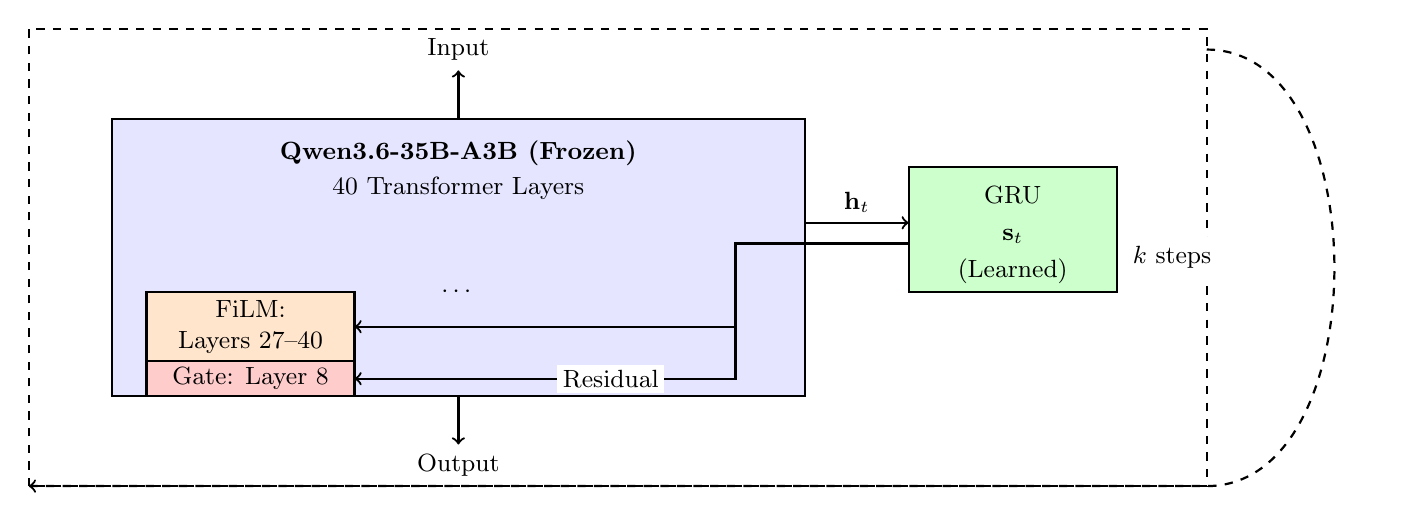
\begin{tikzpicture}[scale=0.88, every node/.style={font=\small}]
% Qwen backbone
\draw[thick,fill=blue!10] (0,0.5) rectangle (10,4.5);
\node[align=center] at (5,4.0) {\textbf{Qwen3.6-35B-A3B (Frozen)}};
\node[align=center] at (5,3.5) {40 Transformer Layers};
\node[align=center] at (5,2.0) {$\cdots$};

% FiLM layers box
\draw[thick,fill=orange!20] (0.5,1.0) rectangle (3.5,2.0);
\node[align=center] at (2,1.5) {FiLM:\\Layers 27--40};

% Gate layer box
\draw[thick,fill=red!20] (0.5,0.5) rectangle (3.5,1.0);
\node[align=center] at (2,0.75) {Gate: Layer 8};

% Input/Output
\draw[->,thick] (5,4.5) -- (5,5.2) node[above] {Input};
\draw[->,thick] (5,0.5) -- (5,-0.2) node[below] {Output};

% GRU + S_t on the right
\draw[thick,fill=green!20] (11.5,2.0) rectangle (14.5,3.8);
\node[align=center] at (13,3.4) {GRU};
\node[align=center] at (13,2.8) {$\mathbf{s}_t$};
\node[align=center,font=\small] at (13,2.3) {(Learned)};

% Backbone h_t to GRU
\draw[->,thick] (10,3.0) -- (11.5,3.0) node[above,midway] {$\mathbf{h}_t$};

% S_t injects back (FiLM)
\draw[->,thick] (11.5,2.7) -- (9.0,2.7) -- (9.0,1.5) -- (3.5,1.5);

% S_t injects back (Gate)
\draw[->,thick] (9.0,2.5) -- (9.0,0.75) -- (3.5,0.75);
\node[align=center,fill=white,inner sep=2,font=\small] at (7.2,0.75) {Residual};

% k-step loop
\draw[dashed,thick] (-1.2,-0.8) rectangle (15.8,5.8);
\draw[->,thick,dashed] (15.8,5.5) to[out=0,in=0] (15.8,-0.8) to[out=180,in=0] (-1.2,-0.8);
\node[align=center,fill=white] at (15.3,2.5) {$k$ steps};
\end{tikzpicture}
\caption{System architecture. A GRU-evolved latent state $\mathbf{s}_t$ modulates a frozen backbone via FiLM (layers 27--40) and gated residual injection (layer 8). The backbone forward pass and GRU update iterate $k$ times per reasoning step.}
\label{fig:arch}
\end{figure}

\subsection{Training Protocol}

We train only the PLAA modules using AdamW (lr $= 10^{-4}$, weight decay $= 0.01$) with 4-bit quantization. Each experiment runs 200--500 gradient steps with batch size 2. The backbone model is loaded in 4-bit (fp4) using bitsandbytes and remains in evaluation mode throughout. All training runs on a single RTX PRO 6000 Blackwell (96 GB VRAM) with 208 CPU cores and 1 TB RAM.

\textbf{Evaluation correctness.} Custom injection layers (FiLM \texttt{scale\_proj}, gate projection) are \emph{not} persisted by PEFT's default checkpoint serialization, a failure mode that can silently evaluate a system against zero-valued modulation weights. We therefore serialize and reload these weights explicitly and verify, before every evaluation, that (i)~\texttt{scale\_proj} was included in the optimizer during training, (ii)~the state-conditioning path is active during the evaluation forward pass, and (iii)~per-token metrics index the last non-padded position via the attention mask rather than a fixed offset. All results below are measured with verified non-zero injection weights. The four-condition design (Section~\ref{sec:clutrr}) additionally guards against this failure: a silently-disabled checkpoint would render the evolved and zeroed conditions indistinguishable, whereas we observe a $94\times$ separation.

\subsection{Intervention Design}

A key methodological contribution of this work is the systematic use of \textit{latent state intervention} rather than retraining or finetuning. Once trained, the latent state $\mathbf{s}_t$ can be manipulated independently:

\begin{itemize}
    \item \textbf{Zeroing:} $\mathbf{s}_t = \mathbf{0}$ disables state modulation while preserving the PLAA architecture's computational graph.
    \item \textbf{Randomization:} $\mathbf{s}_t = \mathcal{N}(0, I)$ tests whether any non-zero perturbation produces effects.
    \item \textbf{Amplitude scaling:} $\mathbf{s}_t \leftarrow \alpha \cdot \mathbf{s}_t$ for $\alpha \in \mathbb{R}^+$ probes the dose-response relationship.
\end{itemize}

This intervention-based approach provides stronger causal evidence than comparisons between separately trained models.

\section{Experiment 1: CLUTRR Relational Reasoning}
\label{sec:clutrr}

\subsection{Setup}

CLUTRR~\cite{sinha2019clutrr} tests multi-hop relational reasoning from short narrative stories. The model receives a sequence of family relationship facts (e.g., ``Clara is the mother of Logan. Logan is the father of Christian.'') and must answer a relational query (``What is Clara to Christian?''). We use the full test set (200 examples) with $\max\_\text{new\_tokens} = 80$ to allow the model's generation to complete. The backbone's thinking mode is disabled to reduce variability in output format.

To isolate the contribution of the trained state from the contribution of the PLAA architecture itself, we compare four conditions on the same frozen backbone:

\begin{enumerate}
    \item \textbf{Base:} No PLAA modules loaded.
    \item \textbf{Zeroed $\mathbf{s}_t$:} PLAA loaded, latent state set to $\mathbf{0}$.
    \item \textbf{Random $\mathbf{s}_t$:} PLAA loaded, latent state sampled from $\mathcal{N}(0, I)$ at each step.
    \item \textbf{Evolved $\mathbf{s}_t$:} PLAA loaded, latent state evolved via trained GRU (Eq.~\ref{eq:gru}).
\end{enumerate}

\subsection{Results}

\begin{table}[t]
\centering
\caption{Four-condition ablation on CLUTRR (200 examples; ACC is top-1 exact-match on the relation label). The evolved state achieves 47.0\% accuracy while zeroed and base conditions both yield near-zero accuracy. Random state produces weak, noisy effects.}
\label{tab:clutrr_four}
\begin{tabular}{@{}lccccc@{}}
\toprule
Condition & ACC & Has rel. & 1-hop & 2-hop & Non-rel \\
\midrule
Base (no PLAA) & 0.0\% & 100\% & 200 & 0 & 0 \\
Zeroed $\mathbf{s}_t$ & 0.5\% & 100\% & 199 & 1 & 0 \\
Random $\mathbf{s}_t$ & 7.0\% & 58.5\% & 98 & 17 & 83 \\
\textbf{Evolved $\mathbf{s}_t$} & \textbf{47.0\%} & 88.0\% & 44 & \textbf{131} & 25 \\
\bottomrule
\end{tabular}
\end{table}

Table~\ref{tab:clutrr_four} presents the four-condition comparison. Several observations emerge:

\begin{observation}[Architecture baseline]
Base and zeroed conditions produce nearly identical behavior. All 200 outputs contain relation words, but exclusively 1-hop relations (``mother'' or ``father''). This indicates that the PLAA architecture itself, when the latent state is zeroed, does not alter the model's output distribution. The 0.5\% accuracy in the zeroed condition is attributable to noise (1/200 samples).
\end{observation}

\begin{observation}[Random perturbation effect]
Random $\mathbf{s}_t$ increases 2-hop outputs to 8.5\% and accuracy to 7.0\%, but at the cost of 41.5\% non-relation outputs. This suggests that arbitrary perturbations can occasionally shift the model into multi-hop regimes, but the effect is weak and accompanied by format degradation.
\end{observation}

\begin{observation}[Evolved state effect]
The evolved $\mathbf{s}_t$ produces 65.5\% multi-hop outputs and 47.0\% accuracy---a 94$\times$ improvement over the zeroed baseline. 88.0\% of outputs remain valid relation words, indicating the state carries structured task information rather than acting as a general perturbation.
\end{observation}

\subsection{Interim Discussion}

The four-condition design supports the interpretation that the trained $\mathbf{s}_t$ carries genuine task-relevant information. The random condition provides a crucial control: if any non-zero state produced similar results, the evolved state's effects could be attributed to non-specific perturbation. Instead, the evolved state produces 5.5$\times$ more 2-hop outputs than the random state while maintaining output format quality (88\% vs. 58.5\% relation validity).

\section{Experiment 2: Dose-Response Intervention}
\label{sec:dose}

\subsection{Rationale}

A strong test of causal influence is whether systematic variation of the intervention produces systematic variation in the outcome. If $\mathbf{s}_t$ carries genuine information, scaling its amplitude should produce a monotonic or structured response, rather than a binary on/off effect.

We apply $\alpha \in \{0.0, 0.25, 0.50, 0.75, 1.0\}$ as a multiplier to the evolved state after the GRU update:
\begin{equation}
    \mathbf{s}_t' = \alpha \cdot \mathbf{s}_t,\quad \text{where } \mathbf{s}_t \text{ is the trained evolved state.}\label{eq:dose}
\end{equation}
All other experimental parameters are held fixed (CLUTRR, 100 examples, $\max\_\text{new\_tokens} = 80$).

\subsection{Results}

\begin{table}[t]
\centering
\caption{Dose-response intervention ($\alpha \cdot \mathbf{s}_t$) on CLUTRR (100 examples). The response is non-monotonic, peaking at $\alpha = 0.75$.}
\label{tab:dose}
\begin{tabular}{@{}ccccccc@{}}
\toprule
$\alpha$ & ACC & Has rel. & 1-hop & 2-hop & 3-hop & Non \\
\midrule
0.00 & 0.0\% & 100.0\% & 100 & 0 & 0 & 0 \\
0.25 & 2.0\% & 100.0\% & 98 & 2 & 0 & 0 \\
0.50 & 30.0\% & 95.0\% & 57 & 36 & 2 & 5 \\
\textbf{0.75} & \textbf{58.0\%} & 95.0\% & 18 & \textbf{75} & 2 & 5 \\
1.00 & 49.0\% & 90.0\% & 18 & 72 & 0 & 10 \\
\bottomrule
\end{tabular}
\end{table}

\begin{figure}[t]
\centering
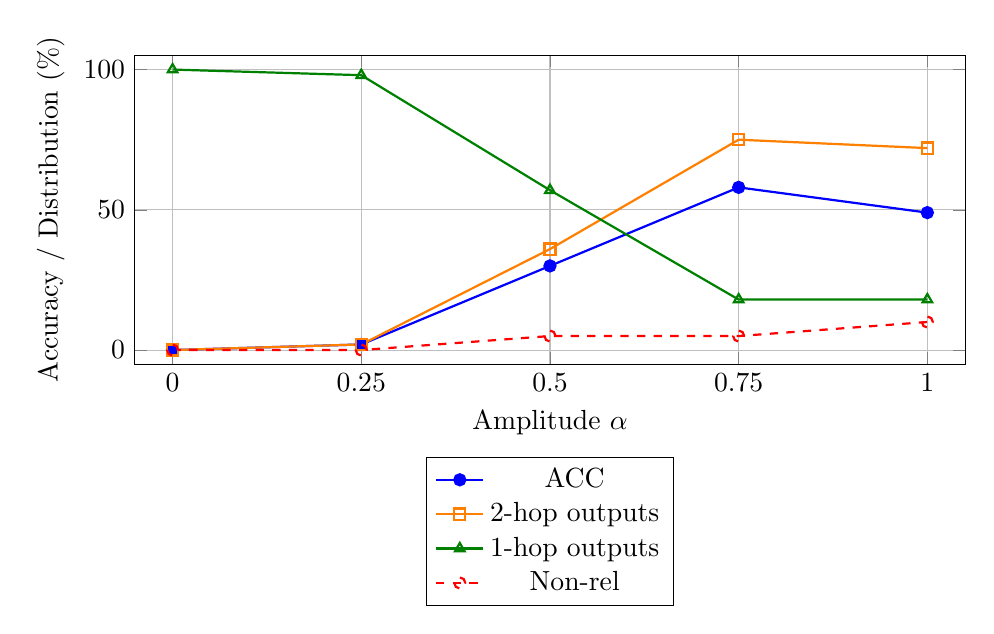
\begin{tikzpicture}
\begin{axis}[
    xlabel=Amplitude $\alpha$,
    ylabel=Accuracy / Distribution (\%) ,
    xmin=-0.05, xmax=1.05,
    ymin=-5, ymax=105,
    xtick={0,0.25,0.5,0.75,1.0},
    grid=major,
    legend style={at={(0.5,-0.3)},anchor=north},
    width=\columnwidth, height=5.5cm]
\addplot[thick,blue,mark=*] coordinates {(0,0) (0.25,2) (0.5,30) (0.75,58) (1.0,49)};
\addplot[thick,orange,mark=square] coordinates {(0,0) (0.25,2) (0.5,36) (0.75,75) (1.0,72)};
\addplot[thick,green!50!black,mark=triangle] coordinates {(0,100) (0.25,98) (0.5,57) (0.75,18) (1.0,18)};
\addplot[thick,red,dashed,mark=o] coordinates {(0,0) (0.25,0) (0.5,5) (0.75,5) (1.0,10)};
\legend{ACC, 2-hop outputs, 1-hop outputs, Non-rel}
\end{axis}
\end{tikzpicture}
\caption{Dose-response curve for $\alpha \cdot \mathbf{s}_t$. Accuracy peaks at $\alpha = 0.75$ before declining, exhibiting an inverted-U shape. 2-hop outputs track closely with accuracy.}
\label{fig:dose}
\end{figure}

Table~\ref{tab:dose} and Figure~\ref{fig:dose} present the dose-response results. The data exhibit three notable patterns:

\begin{observation}[Smooth transition]
The response is not binary. Accuracy increases monotonically from 0\% ($\alpha = 0$) through 2\% ($\alpha = 0.25$) to 30\% ($\alpha = 0.50$), demonstrating that the latent state's influence scales with amplitude.
\end{observation}

\begin{observation}[Inverted-U peak]
Accuracy peaks at $\alpha = 0.75$ (58\%) and declines at $\alpha = 1.00$ (49\%). The full-amplitude state produces more non-relation outputs (10 vs.\ 5 at $\alpha = 0.75$), suggesting that at higher amplitudes the modulation becomes disruptive.
\end{observation}

\begin{observation}[2-hop tracking]
The number of 2-hop outputs closely tracks accuracy (36 at $\alpha = 0.50$, 75 at $\alpha = 0.75$, 72 at $\alpha = 1.00$), confirming that performance gains are driven by successful multi-hop reasoning rather than improved 1-hop guessing.
\end{observation}

\subsection{Analysis}

The non-monotonic dose-response curve is inconsistent with a simple additive signal model. If $\mathbf{s}_t$ were simply adding task-relevant information to the residual stream, larger $\alpha$ should produce monotonically better results. The decline at $\alpha = 1.0$ suggests interference effects: at full amplitude, the modulation may disrupt the backbone's internal representations.

One plausible interpretation (see the Reasoning Attractor Hypothesis, Section~\ref{sec:attractor}) is that $\mathbf{s}_t$ modulates transitions between computational regimes. At low amplitudes ($\alpha \leq 0.25$), the state is too weak to induce a regime shift. At intermediate amplitudes ($\alpha \approx 0.5$-$0.75$), the state partially induces multi-hop reasoning. At full amplitude ($\alpha = 1.0$), the modulation overshoots, causing the model to operate outside its stable regime.

\section{Experiment 3: GSM8K Cross-Turn Reasoning}
\label{sec:gsm8k}

\subsection{Setup}

GSM8K~\cite{cobbe2021training} consists of grade-school math word problems. We split each problem into 3--6 reasoning turns. At each turn, the model receives only the current turn's question (no historical context); $\mathbf{s}_t$ is the only cross-turn information channel. Training uses 4,218 samples with 3+ turns and evaluation on 463 test samples. We train for 500 steps.

\subsection{Results}

\begin{table}[t]
\centering
\caption{GSM8K cross-turn results. Removing $\mathbf{s}_t$ at later training stages causes measurable degradation in both PPL and accuracy.}
\label{tab:gsm8k}
\begin{tabular}{@{}crrrr@{}}
\toprule
Step & PPL$_{\text{with}}$ & PPL$_{\text{without}}$ & $\Delta$PPL & $\Delta$ACC \\
\midrule
100 & 12.71 & 10.18 & $-$2.53 & $-$2.1\% \\
200 & 12.19 & 10.14 & $-$2.05 & $-$1.9\% \\
300 & 10.81 & 10.13 & $-$0.68 & $-$0.4\% \\
400 & 9.58 & 10.11 & $+$0.53 & $+$1.8\% \\
500 & 8.87 & 10.13 & $+$1.26 & $+$2.4\% \\
\bottomrule
\end{tabular}
\end{table}

Table~\ref{tab:gsm8k} shows a clear temporal pattern. At early training (step 100), the randomly initialized $\mathbf{s}_t$ degrades performance relative to ablation ($\Delta$PPL $= -2.53$). As training progresses, the state becomes beneficial. By step 500, removing $\mathbf{s}_t$ \emph{increases} PPL by 1.26 and decreases token accuracy by 2.4 percentage points.

\begin{figure}[t]
\centering
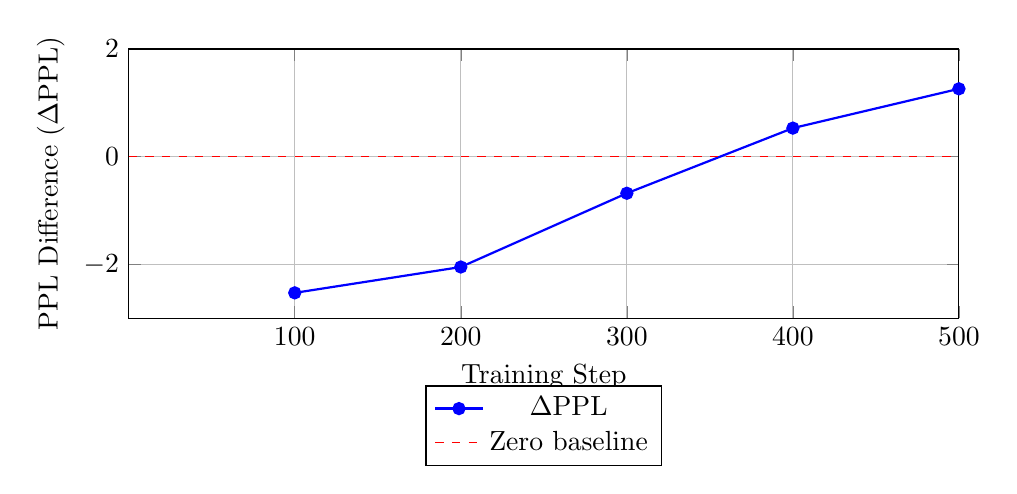
\begin{tikzpicture}
\begin{axis}[
    xlabel=Training Step,
    ylabel=PPL Difference ($\Delta$PPL),
    xmin=0, xmax=500,
    ymin=-3, ymax=2,
    xtick={100,200,300,400,500},
    grid=major,
    legend style={at={(0.5,-0.25)},anchor=north},
    width=\columnwidth, height=5cm]
\addplot[thick,blue,mark=*] coordinates {
    (100,-2.53) (200,-2.05) (300,-0.68) (400,0.53) (500,1.26)
};
\addplot[dashed,red] coordinates {(0,0) (500,0)};
\legend{$\Delta$PPL, Zero baseline}
\end{axis}
\end{tikzpicture}
\caption{GSM8K PPL difference: $\mathbf{s}_t$ transitions from harmful ($-$2.53) to beneficial ($+$1.26) over training.}
\label{fig:gsm8k_ppl}
\end{figure}

\subsection{Analysis}

\textbf{Potential confound.} A notable behavioral side effect of the PLAA architecture became apparent during evaluation: the PLAA framework itself, independent of $\mathbf{s}_t$, alters the model's output mode on GSM8K from generating reasoning text (intermediate steps followed by answer) to producing direct-answer outputs. This architectural effect means that comparison between ``with $\mathbf{s}_t$'' and ``without $\mathbf{s}_t$'' conditions operates within a modified output distribution relative to the unmodified backbone. We include this detail as a transparent confound: the PPL and accuracy deltas in Table~\ref{tab:gsm8k} reflect differences between zeroed and evolved $\mathbf{s}_t$ within the PLAA framework, not between PLAA and the original backbone. The convergent evidence with CLUTRR (where this side effect was not observed, likely because relation-word outputs are less susceptible to output-mode shifts) partially mitigates this concern, but the GSM8K results should be interpreted with this caveat in mind.

The GSM8K experiment provides convergent evidence with the CLUTRR results, but with a weaker effect size. The 2.4\% accuracy delta is modest, which we interpret as consistent with the hypothesis that $\mathbf{s}_t$ carries supplementary cross-turn information rather than dominating the backbone's per-turn inference.

The transition from negative to positive effect is consistent across both metrics (PPL and accuracy flip sign at step 400). We interpret this as: early in training, $\mathbf{s}_t$ adds noise to the backbone's already well-calibrated distribution. As training progresses, the state learns to encode task-relevant cross-turn information that the per-turn backbone cannot access.

\section{Discussion}
\label{sec:discussion}

\subsection{Summary of Evidence}

Taken together, the four-condition ablation (Section~\ref{sec:clutrr}), the dose-response intervention (Section~\ref{sec:dose}), and the GSM8K temporal analysis (Section~\ref{sec:gsm8k}) provide convergent evidence that the trained latent state $\mathbf{s}_t$ exerts measurable causal influence on the model's reasoning behavior. The key findings are:

\begin{enumerate}
    \item The PLAA architecture alone (zeroed $\mathbf{s}_t$) does not affect behavior. The trained state is responsible for the observed effects.
    \item Amplitude scaling produces a non-monotonic, inverted-U-shaped response, inconsistent with simple additive signal models.
    \item Random states produce weak, noisy effects, confirming that the trained state carries structured information.
    \item The GSM8K temporal dynamics show a transition from harmful to beneficial influence, consistent with a learned representation account.
\end{enumerate}

\textbf{Scope of the claim.} The CLUTRR and dose-response results establish that a \emph{trained, state-derived modulation signal} influences reasoning-mode behavior. The stronger claim that this signal carries genuine \emph{cross-turn persistent} state rests primarily on the GSM8K experiment (Section~\ref{sec:gsm8k}), which is subject to the output-mode confound documented there; we therefore treat the cross-turn interpretation as suggestive rather than established.

\subsection{Reconciling with the Near-Inert Regime}

A companion architectural study of the same modulation mechanism on a smaller backbone (Qwen3-4B) reports the opposite headline: under \emph{pure} language-modeling cross-entropy, freezing the latent state changes loss by only $\Delta = 0.0002$ and removing FiLM by $\Delta = 0.044$~\cite{plaa}. We do not regard this as a contradiction, and---given that the compute used here is no longer available---we cannot adjudicate among the following explanations with new experiments; we state them as the live hypotheses:

\begin{enumerate}
    \item \textbf{Metric.} That study measures continuous per-token LM loss on text the backbone already models well (loss $\approx 2.7$); we measure coarse \emph{task accuracy} on CLUTRR, where the unmodulated backbone scores $0\%$ and there is large headroom for any task-aligned signal to register.
    \item \textbf{Regime, not magnitude.} A modulation too weak to perturb a well-calibrated next-token distribution can still flip a \emph{discrete} reasoning-mode decision (1-hop vs.\ multi-hop)---exactly what our dose-response and output-distribution data show.
    \item \textbf{Scale and injection points.} The backbones (35B vs.\ 4B), injected layers (8 and 27--40 vs.\ 16--28), and tasks differ.
\end{enumerate}

We accordingly frame our central claim narrowly: the trained state exerts measurable influence \emph{on reasoning-mode behavior}. This is consistent with---not contradicted by---its near-zero influence on fine-grained LM loss in the smaller-backbone study, and the two findings together delineate \emph{where} bounded latent modulation does and does not register.

\subsection{The Reasoning Attractor Hypothesis}
\label{sec:attractor}

We offer the following as a \textit{tentative interpretation} rather than an established mechanism:

\begin{hypothesis}[Reasoning Attractor]
The backbone model's hidden states, when conditioned on a task-relevant prompt, occupy a high-dimensional landscape with multiple attractor basins corresponding to different computational regimes (e.g., 1-hop vs. multi-hop reasoning). The trained $\mathbf{s}_t$, injected via FiLM modulation and residual connections, shifts the trajectory of hidden states toward the multi-hop attractor basin. At optimal amplitude ($\alpha \approx 0.75$), the modulation cleanly induces the transition. At higher amplitudes, the modulation overshoots, pushing the trajectory into an unstable region.
\end{hypothesis}

This hypothesis is consistent with three observations: (1) the non-monotonic dose-response (the ``Goldilocks'' amplitude), (2) the increased format degradation at $\alpha = 1.0$ (indicating the model is pushed outside its stable operating regime), and (3) the random state's weak but non-zero effect (any perturbation can occasionally cross an attractor boundary by chance).

\textbf{Important caveat.} We emphasize that this is a \textit{post-hoc interpretation}, not a tested prediction. Direct evidence for attractor dynamics would require hidden-state trajectory analysis, which we leave for future work.

\subsection{Limitations}

This study has several limitations that qualify the strength of our claims:

\begin{enumerate}
    \item \textbf{Single benchmark.} The primary dose-response experiment uses only CLUTRR. While GSM8K provides convergent evidence, the benchmark diversity is limited.
    \item \textbf{Single seed.} All experiments use a single random seed (42). The effects may be sensitive to initialization.
    \item \textbf{No layer sweep.} FiLM modulation is restricted to layers 27--40 and residual injection to layer 8. The effect may vary across different layer selections.
    \item \textbf{No negative-amplitude intervention.} We test $\alpha \geq 0$ but not $\alpha < 0$, which would help distinguish between amplitude effects and directional effects.
    \item \textbf{Small-scale architecture.} The latent state dimension is 128; the backbone is a single model. Generalization to larger models and higher-dimensional latents is untested.
    \item \textbf{Post-hoc interpretation.} The Reasoning Attractor Hypothesis is proposed after observing the results. It should be treated as a framework for future hypothesis generation rather than a confirmed mechanism.
\end{enumerate}

\subsection{Future Work}

Several directions follow from this work:

\begin{enumerate}
    \item \textbf{Higher-dimensional latent states.} The current 128-dimensional state may impose informational bottlenecks. Scaling to 512 or 1024 dimensions could improve expressiveness.
    \item \textbf{Layer-wise interventions.} Injecting the state at different layers or with layer-dependent amplitudes could reveal which parts of the backbone are most receptive to modulation.
    \item \textbf{Negative-amplitude experiments.} Applying $\alpha < 0$ would help distinguish whether effects are due to amplitude or to specific directional information.
    \item \textbf{Hidden-state analysis.} Computing trajectory distances or attractor metrics (e.g., via PCA or persistent homology) on backbone hidden states could test the Reasoning Attractor Hypothesis directly.
    \item \textbf{Larger reasoning benchmarks.} Evaluating on BIG-Bench Hard~\cite{suzgun2022challenging} or MuSiQue~\cite{trivedi2022musique} would test generality.
    \item \textbf{Behavioral side effects.} As discussed in Section~\ref{sec:gsm8k}, the PLAA architecture itself can alter the model's output mode on GSM8K. Understanding and mitigating such architectural side effects is important for clean interpretation of latent state intervention experiments.
\end{enumerate}

\section{Related Work}

\textbf{Architectural latent states.} Recurrent memory~\cite{graves2014neural}, Transformer-XL~\cite{dai2019transformer}, and linear RNNs~\cite{gu2022efficiently} introduce persistent states through architectural modifications. Our approach differs by operating entirely through frozen-backbone injection, which allows clean intervention experiments.

\textbf{Activation engineering.} Activation steering~\cite{turner2023activation, rimsky2023steering} and representation engineering~\cite{zou2023representation} modify model outputs by adding vectors to hidden states. Our work extends this paradigm by making the steering signal itself state-evolved, and by providing systematic dose-response evidence.

\textbf{Latent reasoning.} Coconut~\cite{hao2024reasoning} and related work~\cite{deng2023chain} explore internal reasoning without explicit token generation. Our GSM8K experiment aligns with this direction while providing ablation-based causal evidence.

\textbf{Dose-response in AI.} Prior work on intervention strength in activation engineering~\cite{turner2023activation} has noted that scaling intervention magnitudes can produce non-monotonic effects. Our results provide a controlled demonstration of this phenomenon in the context of persistent latent states.

\section{Conclusion}

We present evidence that a learned persistent latent state $\mathbf{s}_t$, injected into a frozen LLM, systematically influences reasoning behavior. The evidence rests on three pillars: a four-condition ablation design showing that the trained state yields 47.0\% accuracy vs.\ 0.5\% for the zeroed baseline; a dose-response intervention producing a non-monotonic inverted-U curve peaking at $\alpha = 0.75$ with 58\% accuracy; and a GSM8K temporal analysis showing the state transitions from harmful to beneficial over training.

These results support the claim that persistent latent modulation of frozen LLMs produces measurable, controllable, and structured influence on reasoning behavior. The non-monotonic dose-response suggests richer dynamics than simple additive information transmission, which we tentatively frame within a Reasoning Attractor Hypothesis.

We emphasize the limitations of this work---single benchmark, single seed, restricted intervention space---and identify clear directions (higher-dimensional states, layer-wise and negative-amplitude interventions, hidden-trajectory analysis) for strengthening the evidence base.

\bibliographystyle{unsrt}
\begin{thebibliography}{20}

\bibitem{graves2014neural} A.~Graves, G.~Wayne, and I.~Danihelka.
\newblock Neural turing machines.
\newblock \emph{arXiv:1410.5401}, 2014.

\bibitem{bulatov2022recurrent} A.~Bulatov, D.~Kuratov, and M.~Burtsev.
\newblock Recurrent memory transformers.
\newblock \emph{NeurIPS}, 2022.

\bibitem{turner2023activation} A.~Turner, L.~Thiergart, and D.~Udell.
\newblock Activation addition: Steering language models without optimization.
\newblock \emph{arXiv:2308.10248}, 2023.

\bibitem{zou2023representation} A.~Zou et al.
\newblock Representation engineering: A top-down approach to AI transparency.
\newblock \emph{arXiv:2310.01405}, 2023.

\bibitem{hao2024reasoning} S.~Hao et al.
\newblock Coconut: Chain-of-thought reasoning without reasoning tokens.
\newblock \emph{arXiv:2406.07137}, 2024.

\bibitem{cobbe2021training} K.~Cobbe et al.
\newblock Training verifiers to solve math word problems.
\newblock \emph{arXiv:2110.14168}, 2021.

\bibitem{sinha2019clutrr} K.~Sinha, R.~Shwartz, and Y.~Goldberg.
\newblock CLUTRR: A diagnostic benchmark for inductive reasoning.
\newblock \emph{EMNLP}, 2019.

\bibitem{cho2014learning} K.~Cho et al.
\newblock Learning phrase representations using RNN encoder-decoder.
\newblock \emph{EMNLP}, 2014.

\bibitem{perez2018film} E.~Perez et al.
\newblock FiLM: Visual reasoning with a general conditioning layer.
\newblock \emph{AAAI}, 2018.

\bibitem{plaa} X.~Ouyang.
\newblock Persistent latent modulation in frozen LLMs: from additive bottleneck to multiplicative symmetry breaking.
\newblock Companion manuscript, 2026.

\bibitem{deng2023chain} Y.~Deng, M.~Emmons, and M.~Liu.
\newblock Chain-of-thought reasoning without chains.
\newblock \emph{arXiv:2311.09256}, 2023.

\bibitem{dai2019transformer} Z.~Dai et al.
\newblock Transformer-XL: Attentive language models beyond a fixed-length context.
\newblock \emph{ACL}, 2019.

\bibitem{gu2022efficiently} A.~Gu and T.~Dao.
\newblock Efficiently modeling long sequences with structured state spaces.
\newblock \emph{ICLR}, 2022.

\bibitem{rimsky2023steering} N.~Rimsky et al.
\newblock Steering language models with activation engineering.
\newblock \emph{arXiv:2308.10246}, 2023.

\bibitem{suzgun2022challenging} M.~Suzgun et al.
\newblock Challenging BIG-Bench tasks and whether chain-of-thought can solve them.
\newblock \emph{arXiv:2210.09261}, 2022.

\bibitem{trivedi2022musique} H.~Trivedi et al.
\newblock MuSiQue: Multi-hop questions via single-hop question composition.
\newblock \emph{ACL}, 2022.

\end{thebibliography}

\end{document}
